\item 
\textbf{Espejos de Fresnel}\\
\begin{minipage}[t][3.75cm]{0.6\textwidth}
Se usa como fuente luminosa para un par de espejos de Fresnel una ranura $D$ iluminada con luz monocromática de \SI{4000}{\angstrom} y colocada a \SI{20}{\centi\metre} de la intersección de los espejos sobre la bisectriz.
Las franjas de interferencia observadas a \SI{1}{\metre}  de distancia del vértice de los espejos tienen una interfranja de \SI{1}{\milli\metre}.
Calcular el ángulo $\alpha$ entre los planos de los espejos.
La distancia vértice-pantalla: \SI{1}{\metre} y $d = \SI{20}{\centi\metre}$.
Note que la fuente y las dos imágenes son equidistantes de la intersección de los espejos. 
\end{minipage}
\begin{minipage}[c][1cm][t]{0.35\textwidth}
	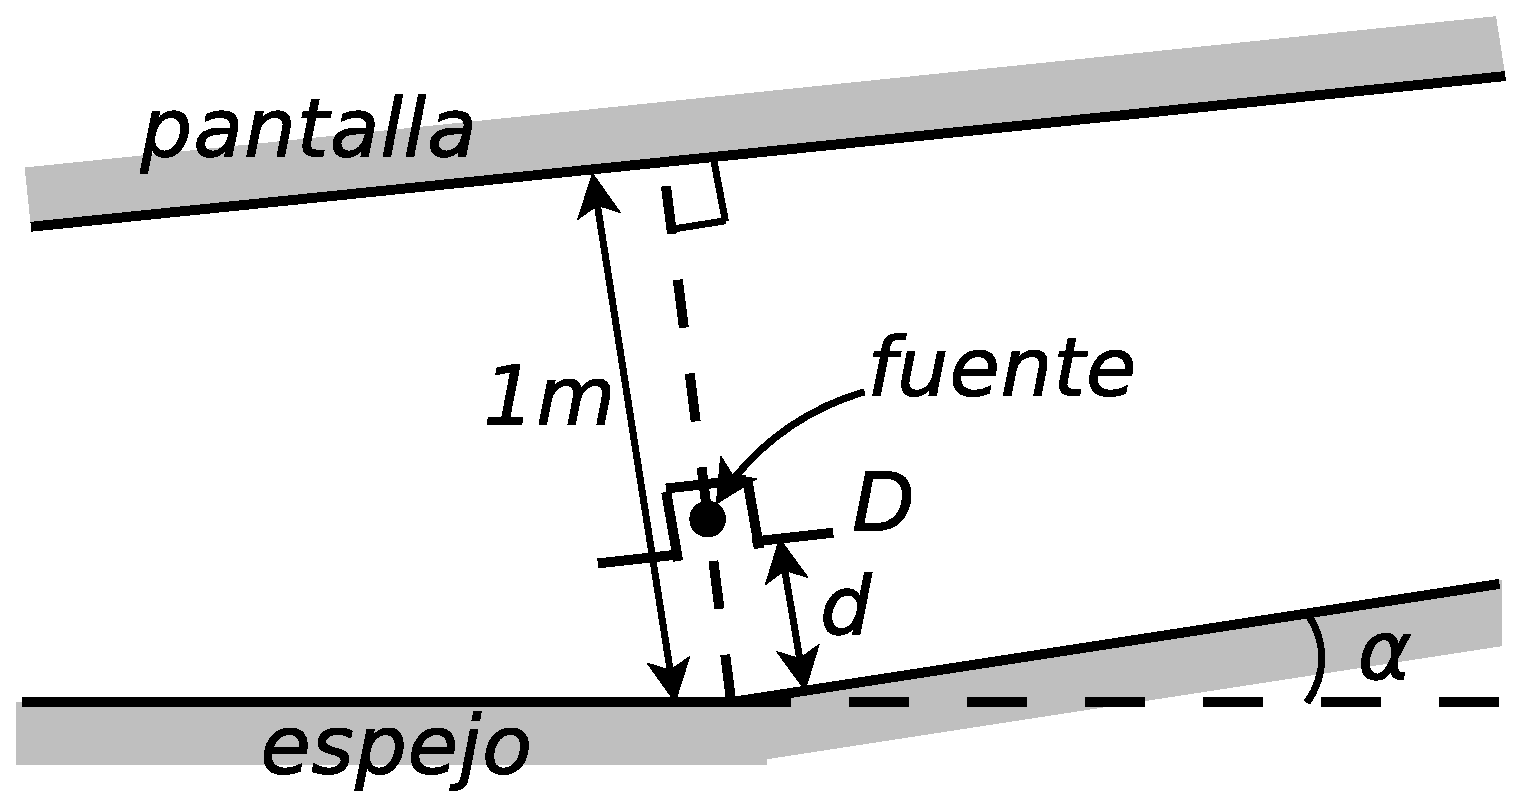
\includegraphics[width=\textwidth]{ej5-8}
\end{minipage}



\item 
\textbf{Espejos de Fresnel | Interfranja}
\begin{enumerate}
	\item En un experimento de interferencia con espejos de Fresnel, ¿qué parámetros deben modificarse para que la interfranja disminuya?
	\item Examinadas con una lupa de distancia focal $f = \SI{5}{\centi\metre}$, dos franjas de interferencia consecutivas, producidas con los espejos de Fresnel, se encuentran a una separación aparente $i' = \SI{3}{\milli\metre}$.
	La distancia entre las imágenes de la fuente y la pantalla es $D = \SI{4}{\metre}$ y la separación entre las dos imágenes es $d = \SI{4}{\milli\metre}$.
	¿En qué longitud de onda emite la fuente?
	Nota: suponer que la imagen de las franjas se forma a una distancia $D_v = \SI{25}{\centi\metre}$ (distancia de visión clara) de la lupa.
\end{enumerate}



\item (*) \textbf{Espejos de Lloyd}\\
¿Por qué motivo se puede concluir, en el experimento del espejos de Lloyd, que la luz reflejada ha sufrido un desfasaje de \ang{180;;}?
